\section{Neural Discrete Representation Learning}

Recent advances in generative modelling of images, audio and videos have yielded impressive
samples and applications. At the same time the challenges that follow these tasks are few-shot
learning, domain adaptation, or reinforcement learning heavily rely on learnt representations from raw data.

Learning representations with continuous features have been used in many previous 
work but discrete representations  are potentially more natural fit for many applications. 
Discrete representations are a natural fit for complex reasoning, planning and predictive learning
(e.g., if it rains, I will use an umbrella).

This concept of discrete representation gave rise to the Vector Quantization-Variational Autoencoder. 
This model relies on Vector Quantization with the combination of Variational Autoencoder framework with 
discrete latent representations through a novel parameterisation of the posterior distribution of (discrete) 
latents given an observation.~\cite{oord2018neural}

\subsection{Vector Quantization - Variational Autoencoder (VQ-VAE)}

VAEs consist of the following parts: an encoder network which parameterised a posterior  
distribution $q(z|x)$ of discrete latent random variables $z$ given the input data $x$, a prior
distribution $p(z)$, and a decoder with a distribution $p(x|z)$ over input data.

Typically, the posteriors and priors in VAEs are assumed normally distributed with diagonal 
covariance. Extensions include autoregressive prior and posterior models, normalising flows, 
and inverse autoregressive posteriors . VQ-VAE uses discrete latent variables which is  
a new way of training, by using vector quantisation (VQ). The posterior and prior distributions are 
categorical, and the samples drawn from these distributions index an embedding table. These embeddings
are then used as input into the decoder network.

\subsection{Discrete Latent Variables}

Let's define a latent embedding space $e \in R^{K \times D}$ where $K$ is the size of the discrete latent space 
(i.e., a $K$-way categorical), and $D$ is the dimensionality of each latent embedding vector $e_{i}$.
Note that there are $K$ embedding vectors $e_{i} \in R ^D$, $i\in{1, 2, ..., K}$.

The discrete latent variables $z$ are then calculated by a nearest 
neighbour look-up using the shared embedding space $e$ as shown in equation \ref{eqn:discrete}.

\begin{equation}
q(z = k|x) =
\begin{cases}
    1 & \text{for } k = \text{argmin}_{j} \| z_{e}(x) - e_{j} \|_{2} \\
    0 & \text{otherwise}
\end{cases}
\label{eqn:discrete}
\end{equation} 

where $z _e(x)$ is the output of the encoder network.

The input to the decoder is the corresponding embedding vector $e _k$ as given in equation \ref{eqn:decoder}
\begin{equation}
    z _q(x) = e _k, \text{where } k= \text{argmin} _j \| z _e(x) - e _j \| _2
    \label{eqn:decoder}
\end{equation}

\subsection{Learning}

\begin{figure}[h]
    \begin{center}
        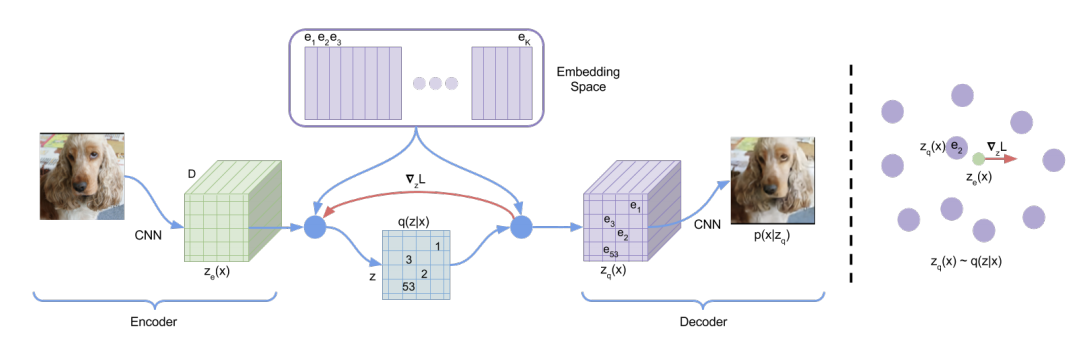
\includegraphics[width=15cm]{vqvae.png}
    \end{center}
    \caption{Left: A figure describing the VQ-VAE. Right: Visualisation of the embedding space. The
    output of the encoder $z(x)$ is mapped to the nearest point $e _2$. The gradient $\nabla _z L$ (in red) will push the
    encoder to change its output, which could alter the configuration in the next forward pass.}
    \label{fig:vqvae}
\end{figure}

During forward computation the nearest embedding $z _q(x)$ is passed to the decoder,
and during the backwards pass the gradient $\nabla _z L$ is passed unaltered to the encoder. 
Since the output representation of the encoder and the input to the decoder share the same $D$
dimensional space, the gradients contain useful information for how the encoder has to change its 
output to lower the reconstruction loss.

As seen on figure \ref{fig:vqvae} (right), the gradient can push the encoder’s output to be discretized 
differently in the next forward pass, because the assignment in equation \ref{eqn:discrete} will be different

The log-likelihood of the complete model $\log p(x)$ can be evaluated as follows:

\begin{equation}
    \log p(x) = \log \sum _k p(x|z _k) p(z _k)
    \label{eqn:modellog}
\end{equation}

Because the decoder $p(x|z)$ is trained with $z = z _q(x)$ from MAP-inference, the decoder
should not allocate any probability mass to $p(x|z)$ for $z \neq zq(x)$ once it has fully converged.

Thus, the authors concluded.~\cite{razavi2019generating, oord2018neural}
\begin{equation}
    \log p(x) \approx \log p(x|z _q(x))p(z _q(x))
\end{equation}

\subsection{Prior}

The author also stated a prior distribution can be made autoregressive by depending on $z$ 
in the feature map as it is a categorical distribution over the discrete latents $p(z)$. 
While training the VQ-VAE the prior is kept constant and uniform. After training, fit 
an autoregressive distribution over $z$, $p(z)$, so that it can generate $x$ via ancestral sampling.
